%% ----------------------------------------------------------------
%% Specification.tex
%% ---------------------------------------------------------------- 
\documentclass{elec6049Report}     % Use the Article Style
%\usepackage{cite}            % Use Natbib style for the refs.
\removecolourlinks    % Uncomment this command to remove colour from any links
%% ----------------------------------------------------------------
%\usepackage[disable]{todonotes}
\usepackage{todonotes}
\usepackage{multirow}
\newcommand{\inote}[1] {\todo[inline]{#1}}
\usepackage{lipsum}
% sets TexCount to ignore inotes
%TC:macro \inote 1
%TC:macro \sect [2]
%TC:macro \subsect [2]

\begin{document}
%TC:ignore
\frontmatter
\reportnumber{1}
\title      {How Does Technology Make Money? - Established Companies}
\authors    {
\texorpdfstring{\href{mailto:hl13g10@ecs.soton.ac.uk}{Henry S. Lovett}}{Henry S. Lovett},
\texorpdfstring{\href{mailto:ajr2g10@ecs.soton.ac.uk}{Ashley J. Robinson}}{Ashley J. Robinson},
\texorpdfstring{\href{mailto:tjs1g10@ecs.soton.ac.uk}{Thomas J. Smith}}{Thomas J. Smith}}

\groupnumber{14}

\maketitle
%TC:endignore
%TC:break Abstract
\begin{abstract}
\inote{An abstract of not more than 200 words is required. It should contain not only a description of the subject and scope of coverage, but also identify the focus of the report.}
\end{abstract}
%TC:break _main_
\mainmatter
% !TeX spellcheck = en_GB
% !TeX root = Report.tex
\phantomsection
\addcontentsline{toc}{section}{Introduction}
\sect{Introduction}

Government legislation pervades all aspects of modern life from welfare to industry, infrastructure to enterprise.
This report is primarily concerned with legislation that governs industry and the pertaining profit potential.
The dictionary definition of legislation is ``laws, considered collectively'' \cite{OED} and the two terms are used synonymously in this report.
One of the main roles of the elected parliament is the debate and passing of new laws or modification to laws.


\begin{figure}[!h]
\centering
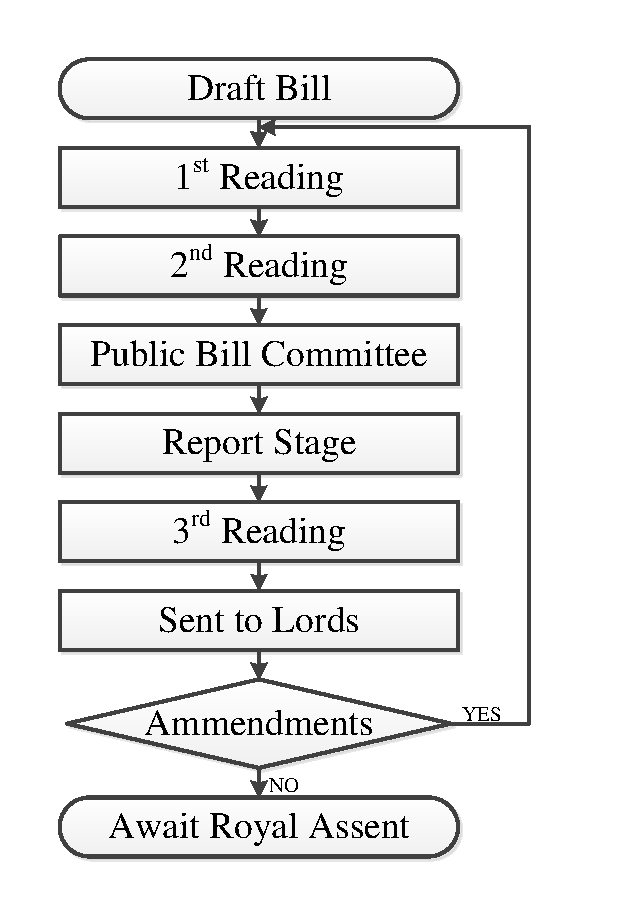
\includegraphics[width = 0.3\textwidth]{Figures/BillFormulation.pdf}
\caption{The passage of a Bill or Act to become Law}
\label{figure:passage}
\end{figure}



% !TeX spellcheck = en_GB
% !TeX root = Report.tex
\phantomsection
\addcontentsline{toc}{section}{Section 1 - Invited Talks}
\sect{Section 1 - Invited Talks} \label{Sect1}
%HSL: I have moved this to the intro
%This section contains a reflection on each of the invited talks in the light of the hypothesis of this report. Full notes from the lectures have been recorded in Appendix 4.

%\phantomsection
%\addcontentsline{toc}{subsection}{Domino Printing Sciences PLC}

\phantomsection
\addcontentsline{toc}{subsection}{Imagination Technologies}
\subsect{Lecture 1}

\lipsum[2]
 



%\phantomsection
%\addcontentsline{toc}{subsection}{ARM}

% !TeX spellcheck = en_GB
% !TeX root = Report.tex
\phantomsection
\addcontentsline{toc}{subsection}{David Parker - Southampton Photonics}
\subsect{Lecture 2 -  David Parker \& Perpetuum}


%\inote{Give a brief intro to them}
Perpetuum are a Southampton based business specialising in energy harvesting modules. 
They were founded in 2004 and they began life as a component supplier for their power module.
\todo[color=red]{Needed?}Perpetuum do not classify as an emerging company in the current day, but the early life of the company and their patent acquisitions are discussed here. 
They are a venture capital funded start-up involving multiple companies.
It was a spin off from a technology developed at Southampton University. 
%\inote{Show Perpetuum is a start up.}

%\inote{Discuss patent acquisitions of Perpetuum}
%http://patents.justia.com/assignee/perpetuum-ltd?page=2
Perpetuum currently hold 22 patents to date. 
Their first was issued on the 23rd August, 2007, some 3 years after they began.
These initial patents prevented any other businesses from being able to reproduce their technology. 
However, the company initially struggled with business.
Their target market was the Oil and Gas industry as they use large drills which vibrate, making it a perfect spot to house their module.
The main issue was that the target market had no application for the module that Perpetuum were attempting to supply. \todo{find out what exactly they were initially supplying}

%In 20xx \todo{find when Parker joined}, David Parker was asked to join Perpetuum. 
Due to the business not fulfilling their potential, they undertook a change. 
The core competencies of the company were considered.
It was easy to see that the main core competency of Perpetuum was in developing energy harvesting modules. 
A second core competence was added to the company of developing a wireless sensor for their module, transferring the product developed from a component, to a system.
This change in focus was accompanied by a change in market - the system was aimed at the transport industry, particularly trains, where there was a gap for a remote monitoring system of the bearings and suspension. 

Even though Perpetuum had a great, novel idea with patents to protect them, it did not make them money by owning the patents alone.
The patents definitely helped, as it meant no other company could have undermined them during the time they were pursuing the non-existent market in oil and gas.
The patents here acted as a barrier to the market, giving them the time to find the correct opportunity to become a success.
Perpetuum have grown rapidly since the shift in core competence and market, with a turn over of around \pounds 2 million in 2013.
There is no doubt that Perpetuum will become ever more successful through the combination of a good idea in the correct market, with patents to protect their product. 

%Another interesting point raised in the lecture by Dr Parker, was that IP is only effective in hardware industry.
%Software is difficult to patent \todo{why is software difficult to patent? Refer to the introduction on patents}

%\inote{Discuss that even though they had patents, they were in the wrong market.}

%\inote{Now they are in a good market, their patents are protecting them and they are doing well.
%Define ``well''. 
%Are they established yet?}

%\inote{Parker briefly spoke about that software is difficult to patent, but hardware is very effective. 
%Results in us looking at hardware companies rather than software.}


%\phantomsection
%\addcontentsline{toc}{subsection}{Imagination Technologies}


% !TeX root = Report.tex
\phantomsection
\addcontentsline{toc}{subsection}{Lecture 3 - Iain Gavin \& Amazon Web Services: HAILO}
\subsect{Lecture 3 - Iain Gavin \& Amazon Web Services: HAILO}

%\inote{Spell checker is up the creek, all my sections need checking - Will do in Soton}





Amazon is, without any reasonable doubt, an established company. 
Founded by Jeff Bezos in 1994 as an online bookshop the company shipped their first book in July 1995~\cite{seattle}. 
The company now has three different parallel business interests. 
The original retail aspect, a 3$^{rd}$ party selling service via the website and Amazon Web Services (AWS).
AWS powers the other two aspects of the business by providing the IT infrastructure that enables such excellent customer service but also acts as an accelerator for other businesses by removing the requirement for on-premises IT solutions. 
They achieve this by maintaining large sever farms from which computing power can be \emph{rented} to facilitate the IT needs of a company. 
They also provide varying degrees of cloud based storage; subject to access latency.

AWS considers a typical split in effort toward a computing heavy business venture, with an on-premises IT solution, to be $30\%$ towards the actual business and $70\%$ towards IT overheads~\cite{gavin2014ams}. 
Their goal is to reverse this distribution by providing the infrastructure for the business. 
One such company that has succeeded using AWS is HAILO~\cite{gavin2014ams}. 
Launched in $2011$ with investments totalling over \$$80$ million from some well known sources such as Union Square Ventures, Accel Partners and Sir Richard Branson~\cite{hailo}.
The company maintains a smartphone app that links customers with the local taxi services however this idea is not unique. 
At the time there was already a large market for smartphone enabled cab rides so something else must have been their source of success~\cite{ventureBeat}. 
Market saturation and a software only product makes patenting redundant so it must have been down to the delivering and quality of the service that has made them a global success. 
Disassociating IT from the business using AWS may well have been a contributing factor to HAILO's ability to concentrate on product delivery.


The Amazon group as whole is very technology driven, the founder filed the first two patents under ``Amazon.Com, Inc'' just before their first sale, and considers innovations as the best method to drive down the prices of the products they sell~\cite{bezos1998secure1,bezos1998secure2}. 
Reasoning behind this idea is shown in Figure~\ref{fig:ScaleInnovation}.
This cycle enables price reduction which naturally improves sales. 
The key step is providing the technology which can improve efficiency therefore staying ahead of competitors. 
Amazon keeps delivering the required technology, patenting aggressively, and at the end of $2013$ created another media buzz by publishing a patent for ``anticipatory package shippin''~\cite{spiegel2013method}!



%\inote{Need to sexify}


\begin{figure}
	\centering
	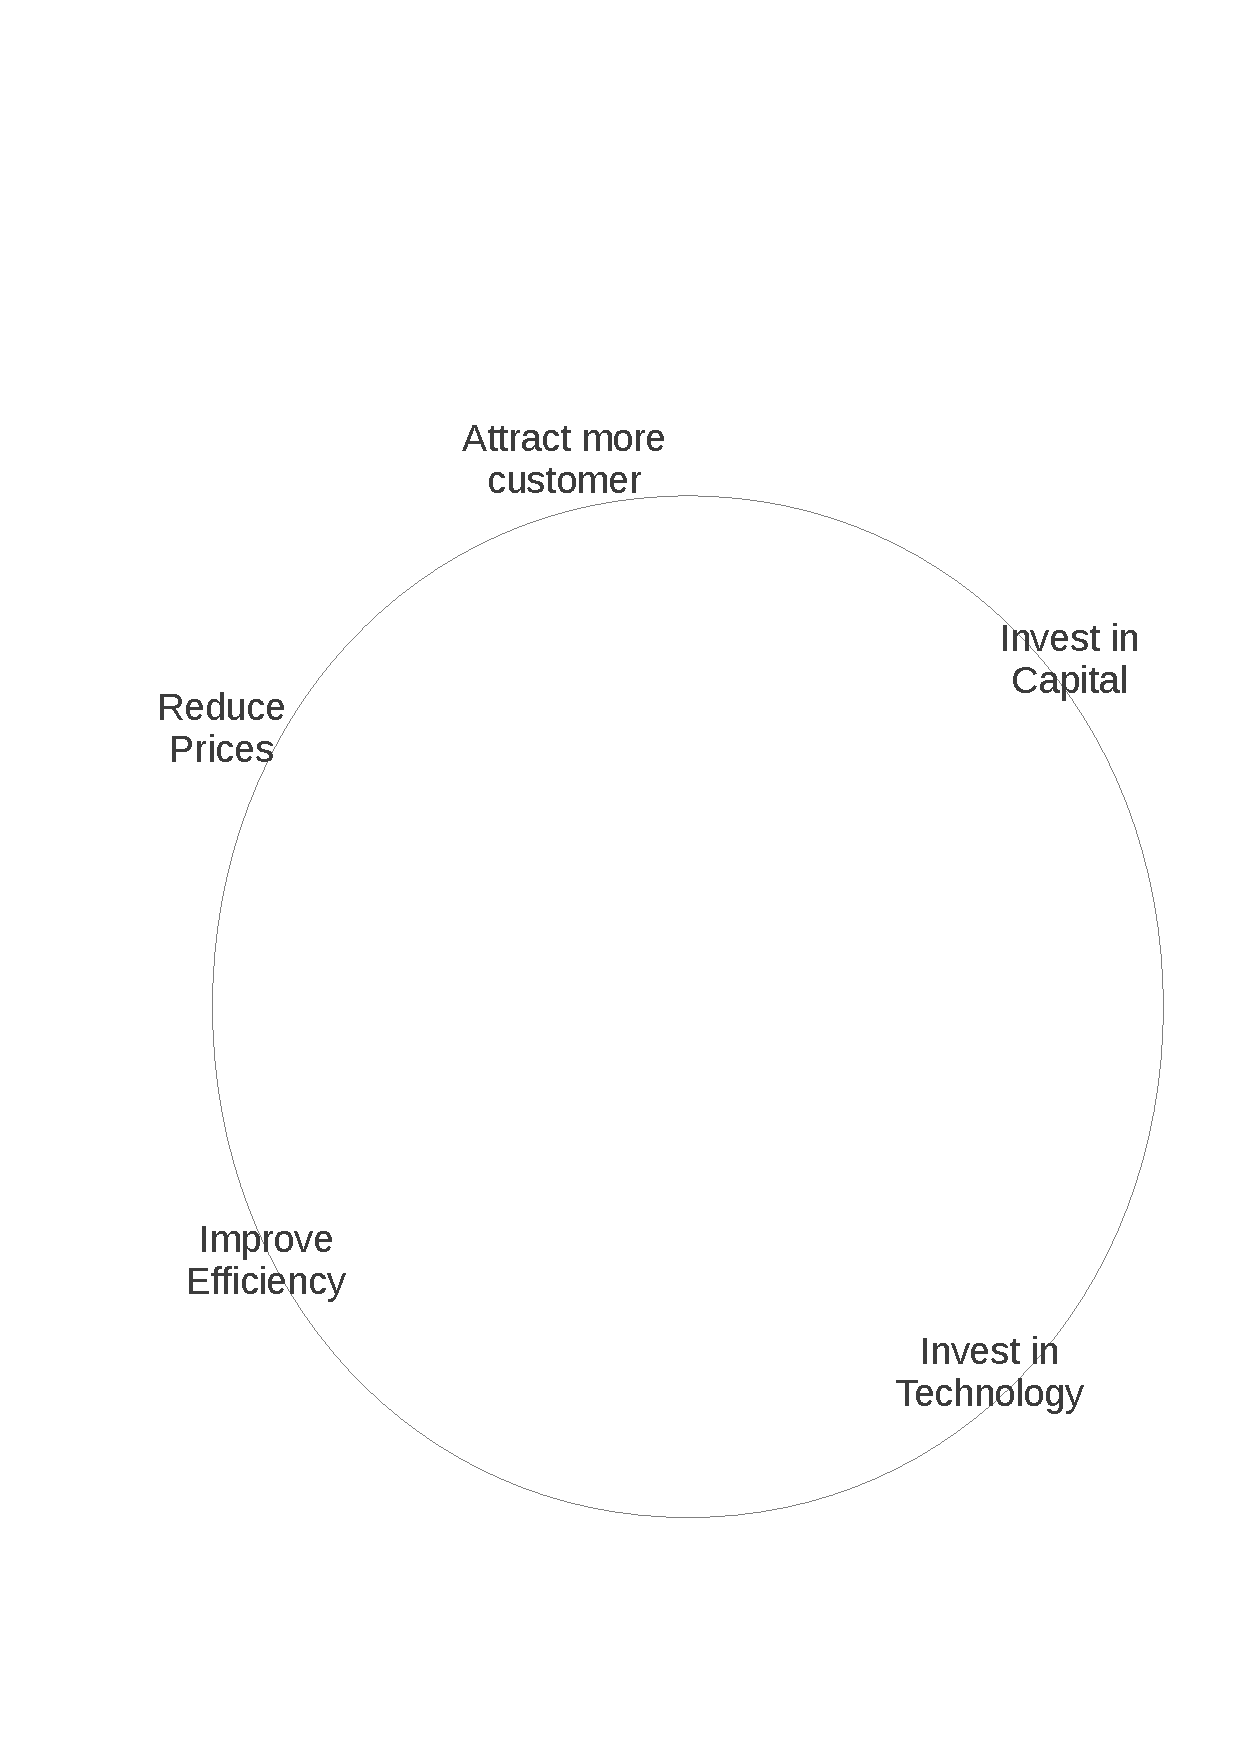
\includegraphics[width=0.4\textwidth]{./Figures/ScaleInnovation.pdf}
	\caption{Scale \& Innovation Drives Down Costs. Taken from~\cite{gavin2014ams}.}
	\label{fig:ScaleInnovation}
\end{figure}



\phantomsection
\addcontentsline{toc}{subsection}{Reflections}
\subsect{Reflection on Common Themes}
\inote{Reflection on Common Themes - HSL I don't think this is needed. We're running out of words and I do summarise all companies in the conclusion. Thoughts? TJS - Agreed. Not really necessary}




% !TeX spellcheck = en_GB
% !TeX root = Report.tex
\phantomsection
\addcontentsline{toc}{section}{Section 2 - }
\sect{Section 2 - }

% !TeX spellcheck = en_GB
% !TeX root = Report.tex
\phantomsection
\addcontentsline{toc}{subsection}{Case1}
\subsect{Nest Labs - Patents for Defence and Value}

Nest Labs was founded in May 2010 by Tony Fadell and Matt Rogers \cite{NestFactsheet}.
The company designs innovative smoke alarms and thermostats that feature iterative learning and are internet connected.
From humble beginnings, Nest have now sold 14 million thermostats and 50 million smoke alarms and employ over 300 people \cite{NestFactsheet}.
The company was acquired by Google for \$3.2bn cash \cite{NestReuters} in February 2014 \cite{NestFactsheet}.
\todo[color=red]{Needed? We've defined already that this means it's a success}Although the company has not yet existed for 8 years, the acquisition by Google makes Nest Labs a successful emerging company.
This case-study will examine the acquisition by Google and ascertain the criticality of patents to the success of this emerging company.

Nest has a strong design heritage, both co-founders were ex-Apple employees and CEO Tony Fadell is widely accredited as the father of the Apple iPod \cite{NestAppleInsider}.
Many Nest employees are also Apple alums \cite{NestReuters}.
This includes Richard `Chip' Lutton, appointed as Vice President and general counsel in 2012 \cite{NestAppleInsider}, who was heavily involved in Apple's patent strategy \cite{NestReuters}.
Nest has a somewhat unusual patent strategy for an emerging company.
Before the Google acquisition Nest had already settled 100 patent disputes \cite{NestCoLabs}.
It also owns 200 patents and has another 200 ready to file \cite{NestCoLabs, NestIV}.
The company signed an agreement with Intellectual Ventures in September 2013 granting access to IV's 40,000 strong patent portfolio \cite{NestIV}.
This is an aggressive approach to patenting, which is not normally pursued by an independent emerging company due to the legal costs \cite{zahra1996technology}.
The expertise gained through some of the employees experience at Apple must play a role in Nest's patenting strategy.

Nest's aggressive patent strategy is partly motivated by defence. 
The company has faced three major patent disputes since it's inception.
Thermostat manufacturer Honeywell filled a lawsuit against Nest for patent infringement in 2012 \cite{NestHoneywellGig, NestHoneywellVerge, NestHoneywell}.
The claims surrounded several patents for technology in Nest's intelligent thermostat.
Although the lawsuit is ongoing \cite{NestFirstVerge}, Nest has largely dismissed these claims, and have stated that Honeywell often use this strategy whenever posed with competition.
As a result of this first lawsuit, Nest hired Richard Lutton and entered the deal with Intellectual Ventures \cite{NestFirstGig}.
Additional patent infringement cases have been filed by First Alert in November 2013 over Nest's intelligent smoke alarm \cite{NestFirstVerge, NestFirstGig}.
Allure Energy are also pursuing a lawsuit for proximity control technology in Nest's thermostat \cite{NestAllureCnet}.
Taking an aggressive approach to patenting will allow Nest to defend itself against these more established companies \cite{NestAllureCnet}.
Disruptive technology such as the Nest thermostat has the ability to transform a marketplace, and stall major revenue streams for incumbants \cite{NestCoLabs}. 
Larger established companies often use the threat of expensive patent litigation to manage the threat of emerging disruptive technology, as Honeywell, Allure and First Alert have in this case study.
While a defence strategy can be expensive, when combined with an appropriate level of expertise and financial backing, an emerging company can adequately defend itself in court, allowing the company to profit from it's technology.

A final area of patent strategy that is evident in this case study, is valuation at exit.
Google has acquired a number of businesses with a focus on extending it's patent portfolio.
Nest marks it's second largest acquisition to date, with Motorola Mobility being the largest \cite{NestReuters}.
Google now owns double the patents it held in 2012 \cite{NestCoLabs}.
This is a result of the patent wars over the Android operating system, which has cost Google 100s of millions of dollars \cite{NestCoLabs}.
The technology Nest Labs develops clearly has a value to Google, and this value lies partly in the 200 patents the company holds.

%\inote{Could also talk about venture capital from here 
%http://techcrunch.com/2014/01/13/nest-investors-strike-it-rich/ 
%But I don't think it is very relevant. Some Venture Capital companies have made 400m dollars on this acquisition and a 20x return in 5 years. If needed I can talk about it.}

%Nest patent litigation with Honeywell and Allure

%Nest patent acquisition by Google





%  Document created by seblovett on seblovett-Ubuntu
%  Date created: Sun 16 Feb 2014 13:54:36 GMT
%  <+Last Edited: Sat 22 Mar 2014 17:43:31 GMT by seblovett on seblovett-Ubuntu +>
% !TeX spellcheck = en_GB
% !TeX root = Report.tex
\phantomsection
\addcontentsline{toc}{subsection}{Atmel}
\subsect{Atmel - Patents not vital to success}


%\todo{Brief intro to atmel.}
%\todo{Show that the classify as a blossoming company during the time we are looking at.}
Atmel Technologies was founded in 1984 by a former Intel employee, George Perlegos.
They were venture capital funded, with only \$30,000 (USD) in initial investment.
Atmel in the current day are a very well established company, with offices in many different countries, multiple product ranges and had a turn over of \$150.93 million (USD) in the last quarter of 2013 \cite{atmel:profit}.
For the purpose of this case study, the early life of Atmel provides a good case study with respect to their patents.


Atmel hold around 1200 patents as of 2014 \cite{atmelpatents} in varying aspects of technology, from touch screen related methods, to fabrication techniques.
Their first patent was issued on 16th May, 1989 \cite{atmel:eprompatent}, 5 years after the company was founded.
In the years previous to their first patent, Atmel encountered patent issues.

In 1987, Atmel were the subject of a patent infringement case from Intel.
Intel claimed that Atmel's ERPOM technology which they were selling to Motorola and Nokia, infringed on the patents they held.
Atmel could have fought a legal battle against Intel, but they chose not to. 
This could have been due to the costs associated with patent litigation, or that Atmel were guilty of infringing on Intel's patents.
%This could have been due to the costs (given that Atmel did not start out with a lot of money, legal costs were likely to have made a detrimental impact on the company), or that Atmel did not have much of a defence.
As Atmel didn't own any patents at this time, it looked like Intel would win the case. 

With hindsight, the decision to not fight the legal battle was the correct one. 
Little money was spent on the proceedings, and it forced Atmel to redesign their EPROM technology.
Their new design turned out to not only out perform Intel's device, it also consumed less power.
Later, this improved memory was included in their microcontrollers, providing an edge in a different market as the EPROM could be included on chip.
Atmel's first patent was about their EPROM fabrication process \cite{atmel:eprompatent}.
This patent was then followed by 3 more that year, all based around their EPROM technology \cite{atmel:eprom1,atmel:eprom2,atmel:eprom3}.

This case study shows that the acquisition of patents is not necessarily a good thing.
If Atmel had gained early patents of their EPROM technology, they may have been more likely to fight a costly patent litigation case against Intel.
Given the little funding Atmel started with, it could have cost them more than money, with time being wasted. 
It could be argued that the initial technology did in fact, infringe on Intel's patents, and could therefore not be patented.
However, due to the financial standings of the company, the costs for both owning and defending a patent were possibly too much at the time.
Even if Intel did not hold patents, and did not prosecute Atmel, the overall success of Atmel could be debatable. 
Their renewed effort on memory devices impacted their later microcontroller memory, of which is now a very large core competence of Atmel.

Since their success with EPROM memory, Atmel received extra funding \cite{atmel:acq1} and purchased foundries to further their R\&D into silicon memories. 
In the modern market, Atmel develop both hardware and software products. 
Their initial success was spurred by not having a defence against someone else's patents. 
In this situation, patents would have not been advantageous to Atmel.




% !TeX spellcheck = en_GB
% !TeX root = Report.tex
\phantomsection
\addcontentsline{toc}{subsection}{Case 3 - 4G Mobile Broadband}
\subsect{Case 3 - 4G Mobile Broadband}


Why the wireless spectrum must be controlled and governed. 

Current allocation of the spectrum

Overview of 4G

Auctioning of the spectrum. 
Who won, what this means.

Why the governance of this makes the dollar, and how it improves/hinders the growth of technology.









\backmatter
\inote{The references so far do not follow the required format. See the word document for the required format. I'm not sure exactly what format it is but it has more information than currently}
\bibliographystyle{unsrt}%{ieeetr}
\bibliography{Report1Bib}

\appendix
%TC:ignore
%  Appendix_Contributions.tex
%  Document created by seblovett on seblovett-Ubuntu
%  Date created: Sun 16 Feb 2014 09:27:55 GMT
%  <+Last Edited: Sun 16 Feb 2014 17:08:45 GMT by seblovett on seblovett-Ubuntu +>

\phantomsection
\addcontentsline{toc}{section}{Appendix 1 - Team Contributions}
\textbf{\uppercase{Appendix}} \par
\sect{1. Team Contributions}

Note that for each report there will be a different chair person.
The chair person is expected to lead the report writing process, including ultimate decision on topic, the allocation of research and the collation of content provided by others. 
Hence it is expected that one team member contribute more per report, thus averaging out over all three reports for the module.
The contribution to the module as a whole will be approximately even from each team member.

\begin{center}
\begin{longtable}{|>{\raggedright\arraybackslash}m{0.2\textwidth} | m{0.75\textwidth} |} \hline
\textbf{Team Member} & \textbf{Contribution} \\ \hline
\endhead
\texorpdfstring{\href{mailto:tjs1g10@ecs.soton.ac.uk}{Thomas J. Smith}}{Thomas J. Smith} 23914254 & Did Something \\ \hline
\texorpdfstring{\href{mailto:hl13g10@ecs.soton.ac.uk}{Henry S. Lovett}}{Henry S. Lovett} 23900091 & Chairperson for this report.  \\ \hline
\texorpdfstring{\href{mailto:ajr2g10@ecs.soton.ac.uk}{Ashley J. Robinson}}{Ashley J. Robinson} 24008346 & Also did something. \\ \hline
\end{longtable}
\end{center}
%\inote{AJR and HSL fill in your student number - Done}


% !TeX spellcheck = en_GB
% !TeX root = Report.tex
\phantomsection
\addcontentsline{toc}{section}{Appendix 2 - Minutes from Kick-off Meeting}


\sect{2. Meeting Minutes - Report 3 Kick-Off Meeting}
\begin{center}
\begin{longtable}{| m{0.2\textwidth} | m{0.6\textwidth} |} \hline
\textbf{Purpose} & Report 3 Kick-Off Meeting \\ \hline
\textbf{Date and Time} & Monday 5th May 2014 \\ \hline
\textbf{Venue} & 3rd floor Zepler Building, Highfield Campus \\ \hline
\textbf{Participants} & HSL (Henry Lovett), AJR (Ashley Robinson),TJS (Tom Smith)\\ \hline
\textbf{Apologies} &None \\ \hline
\multirow{4}{*}{\textbf{Agenda}} & Assign Chair for this report. \\
  & Review hypothesis. \\
 & Review work done by TJS. \\ 
 & Assign work for report. \\
 & Plan report population timescale. \\
 & Agree date and time of next meeting. \\ \hline
\end{longtable}
\end{center}

\subsect{Minutes of the Meeting}
\begin{center}
\begin{longtable}{| p{0.05\textwidth} |>{\raggedright\arraybackslash}p{0.15\textwidth} | p{0.5\textwidth} |>{\raggedright\arraybackslash}p{0.175\textwidth}|} \hline
\textbf{ID} & \textbf{Subject} & \textbf{Notes and Discussion} & \textbf{Action} \\ \hline
\endhead
1.0	&	Chair	&	AJR as he is the remaing member yet to chair. 	&   -	 \\ \hline
2.0 & Hypothesis & Alignment with governance positively influences potential profit. & - \\ \hline
3.0	&	Review TJS & All agree on chosen case study topic, writing lacks references but otherwise good. & \textbf{TJS 1.0} \\ \hline
4.0 & 	Assign work & TJS to carry on with case study on new-nuclear and write up Alstom lecture. HSL to investigate mobile network governance and write up Tim Whitcher lecture. AJR to investigate rail governance (HS2 or Crossrail) and write up Dr Peter Hatto lecture.   &  \textbf{ALL 2.0} \\ \hline
5.0 & Timescale  & The group is operating more efficiently so aim for a submission immediately after last lecture.  & -\\ \hline
6.0 & Next meeting & Approximately 1 week.  & - \\ \hline

\end{longtable}
\end{center}

\subsect{Action List}
\begin{center}
\begin{longtable}{| p{0.05\textwidth} | >{\raggedright\arraybackslash}p{0.15\textwidth} |  p{0.5\textwidth} | >{\raggedright\arraybackslash}p{0.175\textwidth}|} \hline
\textbf{ID} & \textbf{Action} & \textbf{Comments} & \textbf{Status} \\ \hline
\endhead
1.0	&	Tidy up section.	&		& Open 5th May \\ \hline
2.0	&   Write the report.	&	As quick as possible to enable fast submission due to exams.&	Open 5th May \\ \hline
\end{longtable}
\end{center}








\sect{3. Meeting Minutes - Report 3 Meeting}
\begin{center}
\begin{longtable}{| m{0.2\textwidth} | m{0.6\textwidth} |} \hline
\textbf{Purpose} & Report 3 Final Meeting \\ \hline
\textbf{Date and Time} & Tuesday 13th May 2014 \\ \hline
\textbf{Venue} & BLD 44/2103, Highfield Campus \\ \hline
\textbf{Participants} & HSL (Henry Lovett), AJR (Ashley Robinson),TJS (Tom Smith)\\ \hline
\textbf{Apologies} & None \\ \hline
\multirow{3}{*}{\textbf{Agenda}} & Review work done. \\ 
  & Look forward to submission and make a handin date. \\
  & Next meeting.\\  \hline
\end{longtable}
\end{center}

\subsect{Minutes of the Meeting}
\begin{center}
\begin{longtable}{| p{0.05\textwidth} |>{\raggedright\arraybackslash}p{0.15\textwidth} | p{0.5\textwidth} |>{\raggedright\arraybackslash}p{0.175\textwidth}|} \hline
\textbf{ID} & \textbf{Subject} & \textbf{Notes and Discussion} & \textbf{Action} \\ \hline
\endhead
1.0	&	Work done	&	Very good. AJR required to finish case study and &   \textbf{AJR 1.0}	 \\ \hline
2.0 & Submission  & Set for Sunday 18th May 18:00 &  \textbf{AJR 2.0} \\ \hline
3.0 & Next meeting &  Day before handin. & - \\ \hline

\end{longtable}
\end{center}

\subsect{Action List}
\begin{center}
\begin{longtable}{| p{0.05\textwidth} | >{\raggedright\arraybackslash}p{0.15\textwidth} |  p{0.5\textwidth} | >{\raggedright\arraybackslash}p{0.175\textwidth}|} \hline
\textbf{ID} & \textbf{Action} & \textbf{Comments} & \textbf{Status} \\ \hline
\endhead
1.0	&	Finish case1 and lecture 3.	&	& Open 13th May \\ \hline
2.0	&	Handin Sunday 18th May 18:00.	&	&	Open 13th May \\ \hline
\end{longtable}
\end{center}







\sect{4. Meeting Minutes - Report 3 Final Meeting}
\begin{center}
\begin{longtable}{| m{0.2\textwidth} | m{0.6\textwidth} |} \hline
\textbf{Purpose} & Report 3 Final Meeting \\ \hline
\textbf{Date and Time} & Saturday 17th May 2014 \\ \hline
\textbf{Venue} & 3rd floor Zepler Building, Highfield Campus \\ \hline
\textbf{Participants} & HSL (Henry Lovett), AJR (Ashley Robinson),TJS (Tom Smith)\\ \hline
\textbf{Apologies} & None \\ \hline
\multirow{3}{*}{\textbf{Agenda}} & Review work done. \\ 
  & Look forward to submission and make a handin date. \\
  & Next meeting.\\  \hline
\end{longtable}
\end{center}

\subsect{Minutes of the Meeting}
\begin{center}
\begin{longtable}{| p{0.05\textwidth} |>{\raggedright\arraybackslash}p{0.15\textwidth} | p{0.5\textwidth} |>{\raggedright\arraybackslash}p{0.175\textwidth}|} \hline
\textbf{ID} & \textbf{Subject} & \textbf{Notes and Discussion} & \textbf{Action} \\ \hline
\endhead
1.0	&	Work done	&	Very good. AJR required to finish case study and &   \textbf{AJR 1.0}	 \\ \hline
2.0 & Submission  & Set for Sunday 18th May 18:00 &  \textbf{AJR 2.0} \\ \hline
3.0 & Next meeting &  Day before handin. & - \\ \hline

\end{longtable}
\end{center}

\subsect{Action List}
\begin{center}
\begin{longtable}{| p{0.05\textwidth} | >{\raggedright\arraybackslash}p{0.15\textwidth} |  p{0.5\textwidth} | >{\raggedright\arraybackslash}p{0.175\textwidth}|} \hline
\textbf{ID} & \textbf{Action} & \textbf{Comments} & \textbf{Status} \\ \hline
\endhead
1.0	&	Finish case1 and lecture 3.	&	& Open 13th May \\ \hline
2.0	&	Handin Sunday 18th May 18:00.	&	&	Open 13th May \\ \hline
\end{longtable}
\end{center}

%\clearpage
%  Appendix_LectureNotes.tex
%  Document created by seblovett on seblovett-Ubuntu
%  Date created: Sun 16 Feb 2014 09:34:23 GMT
%  <+Last Edited: Sun 16 Feb 2014 09:35:47 GMT by seblovett on seblovett-Ubuntu +>

\phantomsection
\addcontentsline{toc}{section}{Appendix 5 - Notes from Invited Presentations}
\sect{5. Notes from Invited Presentations} \label{Notes}
These notes are raw and not altered in any way from when they were taken from the invited presentation. These notes have been distilled and focussed through the lens of our report title and hypothesis to the content shown in section 1.
\subsect{Domino Printing Sciences PLC - Carl Reynaud - Director of Hardware Development}
Success - ``bringing new products into market and making a profit.''
The key question for any business is how to make profit in a sustainable manner. You need to be able to make profit, then keep on making a profit.

Background to Domino Printing - mission statement - we will achieve market recognition as the first choice global provider of coding, marketing and variable printing solutions delivering convenience, security and peace of mind. Key markets for Domino include;
\begin{itemize}
\item Date coding packaging - Slippery surfaces requires special technology.
\item Industrial printing and coding - this is on fast moving, small and hot plastics and requires a similar technology to date coding.
\item Printing and Mailing - Completely different technology required to the other two market areas.
\end{itemize}

Domino started with a key breakthrough technology in inkjet printing. This has led to diversification into laser and multijet technologies. The head office is in Cambridge. Domino manufacture around 1000-10,000 products per year, making it a low-medium volume business. This presents a number of challenges and opportunities. The technology portfolio ranges from ideas to mature technologies.

``Most ideas take 20 years to become an overnight success'' - Paul Saffo.

Four key points:
\begin{itemize}
\item You want what?
\item Celebrating Diversity
\item No absolutes
\item Keep updating the toolbox
\end{itemize}

You want what highlights that people are often the forgotten ingredient. It is key to know your customer. The customer often lacks the ability to articulate the problem properly and also lacks the vision to see the solutions. Identify what the customer really values (not necessarily the same as what they say they value) and why that is the case, as that is what customers will pay for. As an engineer, just because it is possible doesn't mean we should do it. Does the world need a better mouse trap? There is a significant skill in being able to capture and distill customer values and then apply that to a practical concept. A practical example was given of a customer specification asking for a printer weighing less than 25kg. Asking why this was the case broke the specification down to a real world requirement, that the printer should be able to be installed by one person to minimise installation costs. This requirement requires far more consideration than just weight and concerns shape, handling, regulation (lone working) and other factors. This is called a 5Y process. Another useful model to follow is the V-model.

Celebrating Diversity - don't try to put in what nature left out. changes in culture, education adn psychology. We need to identify how to work best with each other as a team. This involves knowing how you personally work, and identifying how others you work with behave so that you make best use of the diverse skillset in your team. Meyers Briggs type indicators are often used here. Diversity is particularly important when considering foreign markets. 

No absolutes - there will always be variations, but what is the failure zone. Process capability - understand variance. Need to identify suitable margins of error. Test products to make them fail - don't let the customer have a failed product as that can be disasterous. 

Keep updating the toolbox - Pareto and the 80:20 rule was mentioned, identify the 20\% of the work that delivers 80\% of the value etc. Failure mode effect and analysis provides a framework for risk analysis. 

%\inote{Questions and Answers (Ashley)}

Question and answer session:

"What's the biggest barrier you have encountered as an engineer?" - 
Not understanding how to apply technology as such to make it valuable for the customer. 

"How do the features of an engineering product relate to its success?" - 
Good products tend to have less features. 
It may be the case that less time can be spent fixing a parameter by researching customer preferences than implementing parameter adjusting functionality.
For example take the iPad versus a laptop.
Older generations will choose an iPad because there are less features therefore making it simpler to operate.

"Does Domino have any plans for expansion?" - 
We are currently invested in date code printing but are making a move to variable surface printing and also the printing of different materials.

"You mentioned how knowing your customer was important. How could a business suceed with emrging technologies when no record of the customer is already known?" -
There may exist parallel markets which can give some confidence of an expected customer base.
Focus groups and trade shows are a good way to test new technologies without fully deploying any products.
Constantly requesting customer input is also a good way to update the possible requirements which would lead to the design of a sucessful product.

"How do you measure success?" -
I look at technical forums where customers seek solutions to problems.

"Does domino have any plans to takeover smaller businesses?" -
Not at the present.
We tend to look for businesses that are making a profit rather the businesses which are producing future possible technologies.

"Have you thought of diversifying by making components you would otherwise outsource?" - 
Some of our print heads are brought in because the piezo electronics is too complicated for us to invest resources.
The mounting mechanisms however are designed internally but built externally. 
This allows to retain the intellectual property but not get involved with the machining required for implementation.
We look internally for skills that already exist onto which we could diversify rather than jumping to a completely new business. 

%%%%%%%%%%%%%%%%%%%%%%%%%%%%%%%%%%%%%%%%%%%%%%%%%%%%%%%%%%%%%
%% ARM LECTURE NOTES
%%%%%%%%%%%%%%%%%%%%%%%%%%%%%%%%%%%%%%%%%%%%%%%%%%%%%%%%%%%%%
\subsect{ARM - John Biggs - Senior Engineer}
John has been at ARM since 1986 and helped form ARM in 1990. 
ARM - The architecture of a digital world.
ARM is the worlds leading semiconductor IP company with 30 million processors entering the market every day.
Over 50 billion ARM chips have been shipped to date, 10 billion of which in 2013. 
A major driver is the mobile revolution, with smartphones and tablets vastly outselling desktop machines.

Acorn was founded on 5th December 1978 by Hermann Hauser and Chris Curry. 
Their first contract was to develop fruit machine hardware, to replace the conventional electromechanical solutions. 
The Acorn system 1 was sold for 70 pounds in 1979 based on the 8 bit 6502 processor. 
Acorn's next big hit was the BBC Micro in 1982. 
Chris Curry told the BBC that they would have a working prototype within a week, and the Acorn team just about managed to build it in time. 
Having won the BBC Micro contract, Acorn went on to make a number of other 6502 based machines, including the Electron and Master.

Acorn needed a more powerful computer, and looked to Intel to license the 80286 processor, which was refused. 
As a result Acorn's advanced R\&D labs was set up to build Acorn's own 32-bit processor. 
In 1983, Acorn engineers were inspired by a trip to the Western Design Centre. 
The small scale of this operation gave Acorn confidence to design their own chip. 
Hermann gave the design team two key advantages. 
There was no money, and no people for the project meaning the design had to be simple and elegant.

The first ARM silicon was built in 1985 with 3 micron technology, 25k transistors, 6MHz and less than 0.1W power. 
This was the worlds first commercial available RISC processor. 

To reduce the cost of a home computer, Acorn continued to design further chips, memory controller, video controller and IO controller which were assembled onto a single board. 
These were eventually launched as the Archimedes in 1997.

PDAs started to emerge around 1988 based around portability and handwriting recognition.
Low power chips were required, and Hermann asked ARM to develop an especially low power chip. 
Around the same time, Apple were developing the Newton Message Pad based around the AT\&T Hobbit processor.
In the end they swapped it for the ARM chip, using the ARM610. 
In a bizarre twist of fate the machine designed by Hermann and the Apple device swapped processor. 
The ARM610 was made from 1.2 micron technology and some 358 thousand transistors.

In 1997 ARM was founded as a joint venture with Acorn and Apple, since Apple required to have control over their IP. 
Apple put in 1.5 million pound capital, and Acorn supplied the people and the IP (valued similarly). 
Acorn was financially troubled during the 1980s, and were trying to sell the research group any way. 
So the ARM spin out was mutually agreeable. 
Robin Saxby was decided to be the CEO of the ARM spin out, after meeting him in a pub. 

ARM took some of the benefits of RISC architectures and attempt to reduce costs. 
Robin Saxby was initially advised not to work for ARM as "joint ventures never work". 
He performed a simple SWOT analysis and identified some of the key areas of value in ARM. 
Robin took some of the engineers and promoted them to commercial roles. 
The early years were not easy, 92 featured a company wide pay freeze. 

Robin Saxby - \emph{"If you aren't making mistakes you aren't trying hard enough"}.

Robin developed the partnership model. 
Did he grow ARM until it was acquired by a larger company, grow to become a semiconductor company in its own right or become more embedded with Apple? 
Robin did none of these, and developed the licensee/royalty partnership model. 

The first licensee was with GEC and Sharp. 
GEC were in Portsmouth, and Sharp in Japan which meant they were geographically separate. 
Next the automotive part of TI and Samsung also became a licensee. 
By 1995 ARM started to gain international recognition due to this model, despite there was only 40 people actually working for ARM. 
It was the leverage provided by the partners that made the difference.

The early licenses were perpetual licenses. 
As time progressed, further license terms were developed. 
Term licenses allowed a time limited version of the perpetual license, and there were also several other types. 

1993 - ARM was 3 years old when Nokia approached TI to build a new chipset based on the ARM 7. 
But the footprint was too large due to large 32-bit instruction set. 
The ARM7TDMI was built with a high code density for the mobile phone market. 
This had 170 licensees and shipped over 10 billion of these.
It took until 1996 for the product to enter the market, the Nokia 8110.
Innovative layout techniques were developed which helped this processor be so successful.

In 1998 ARM was a 27 million pound business with a net income of 3 million pounds. 
It was time to float the company in April 1998. 
The stocks soared, and ARM became a billion dollar company overnight. 
The acronym was also dropped at this point.

IP deployment has 3 players, the creator, implementor and integrator. 
A key change in the process was handing over soft IP, so that the implementor developed the processor from RTL to a final design. 
This was driven by the consumer. Developments in logic synthesis meant that soft IP was becoming favorable in terms of flexibility and time to market.
ARM developed a reference methodology to minimise the effort to integrate this soft IP into their product, depending on the required features. 
ARM needed to completely change their technology in order to take advantage of synthesisable cores. 
This became the foundation for the ARM9 and others.

In 2000 the ARM926E was developed which is one of ARMs most successful processors selling over 5bn units. 
The ARM instruction set has had to develop considerably to allow some of the more advanced and extended features. 
Eventually the ARM processors were divided into three families, focusing on different aspects.

2008 saw the ARM Cortex-A9 which was a step forward in multicore processing. 
This was driven by consumers wanting ever more advanced user experiences in mobile devices but also with longer battery life. 
2011 saw the Cortex-A15 which developed the idea of big-little connected by a coherent cache. 
This allowed energy savings of approximately 70\%. 

Looking to the future, a new generation of computing is set to take hold. 
Currently we are in the Mobile Internet phase, but soon entering The Internet of Things phase. 
The Cortex-M0 was built in 2012 which is the most energy efficient 32-bit processor ever built. 
It is aimed at low power IoT applications, such as wireless sensor nodes etc. Much more compact design. 
Freescale produced a processor based on this technology that measures just 2mm square, for ideas such as ingestible electronics.

ARM and ECS at Southampton started a joint research project in 2008.
 Mostly the work is based in the area of energy efficiency. 
The first PhD student has just graduated.

John then made some reflections on how things have changed at ARM. 
Synthesis tools have improved implementation time from 6 months for the ARM1 to just 30 minutes with the Cortex-M0. 
This is in-keeping with Moore's Law. 
Area scaling follows similarly. 
Performance and Voltage do not follow Moore's Law due to the laws of physics. 
However, Power Efficiency has also managed to be increased with Moore's Law. 
ARM is also now a much more global company and is much more connected. 
A couple of extreme examples is a $1 mm^2$ implementation of the Cortex-M0. 
At the other end is a $1 km^3$ computer for neutrino monitoring in the Arctic. 
There is a huge diversity in application. 

ARM servers are now increasingly important, and represent a huge opportunity for ARM. 
ARM's partnership model is paying off in this area as companies seek to produce micro servers that save huge amounts of space, cooling and energy. 
This saves around half the cost of a conventional data sensor.

A world where all electronic products and services are based upon energy efficient technology from ARM, making life better for everyone.

Key lessons:
\begin{itemize}
\item Top-right isn't everything
\item Design once, use many times
\item The partnership is everything
\item Listen to your customer, and their customer
\item Timescales are long
\item People are the biggest asset we have
\item It pays to be different
\item Strive for simplicity beyond complexity.
\end{itemize}

Alan Perlis - \emph{``Fools ignore complexity; pragmatists suffer it; experts avoid it; geniuses remove it!''}

Questions:
Why so many offices - culturally it is better to go and meet the customer face to  face.
Is it beneficial to invest in companies attributed to ARM - No, focusing on licensing and royalty model.
Is the ARM-ECS relationship important - increasingly so. ARM investing in lots of areas, science museums and Raspberry Pi as corporate social responsibility.
What point did ARM feel established and secure in the market - 1996 a guy from Samsung asked if he could come and speak to ARM partners, and he gave the motivational speech.
How important is the mobile sector - It was integral to the business, but now ARM is in so many different market areas.
What makes ARM unique - The partnership model is critical. Defends against aggressive take over from big players like Intel.
Are ARM considering buying any other companies - yes ARM bought Mali graphics just a few years ago that compete heavily with imagination technologies.
How do ARM deal with competing with Imagination and Mali - Issues are more to do with Synopsis as you need synopsis to build these soft cores, but they also have their own IP which can make working together difficult at times.


%%%%%%%%%%%%%%%%%%%%%%%%%%%%%%%%%%%%%%%%%%%%%%%%%%%%%%%%%%%%%
%% IMAGIGAYTION LECTURE NOTES
%%%%%%%%%%%%%%%%%%%%%%%%%%%%%%%%%%%%%%%%%%%%%%%%%%%%%%%%%%%%%
\subsect{Imagination Technologies - David Knox - Senior Director Software Engineer at Ensigma Communications IP}
Talk is entitled Software Defined Radio for Consumer Products. 
High volume consumer products influence our aspirations for technology. 
Who are Imagination Technology? 
Imagination are a leading silicon, software and cloud IP provider. 
They mainly focus on high volume products. 
They also own PURE digital radios which do manufacture a product. 
The city say that PURE should be sold off, but the reason for having it is not necessarily to make money, but give a direct showcase for imaginations IP directly in the market.
 This makes their marketing and licensing of IP much easier. 
They operate in graphics, video, general purpose processors, communications and cloud products. 

Big global company. 
UK is the global HQ with four R\&D facilities. 
Imagination aim to provide SoC IP for every market. Imagination can provide all of the comms, graphics, MIPS CPU and VPU as licensed technology.
 Imagination have licensees but also sell directly to the OEMs, which is a slightly different model to ARM. 
Perhaps this is a sign that the licensees (silicon manufacturers) are some what out of touch with the end consumer of products. 
Licensees vary hugely in size, location and industry. Imagination also engage with the end users as mentioned. 
Technology is used in a huge amount of products, 5 billion products, 3 million products shipped per day. 
Imagination is also trying to drive new technology.

Looking wider in the electronics industry, devices are becoming smarter. 
Everything is intelligent and customisable and connected. 
The Internet of Things is starting with around 10bn plus which is an order bigger than the mobile market. 
Wearable electronics is starting to take off. LTE further liberating smart phones. 
4k screen resolutions are starting to appear. 
Variety of processors, MIPS, ARM and Intel.

The market in communications is too fragmented. 
There are too many standards worldwide. 
Different trade offs need to be made for each standard. 
The standards are likely to not be consolidated due to this, as they all do different jobs. 
There seems to be no one size fits all strategy. Additionally, there is the power of world politics at play. 
If you want a worldwide product you have to support many many different communications protocols, consider mobile phones as an example. 
Additionally, more products are becoming connectable. 

The Internet of things will permeate everywhere, central heating, thermostats, lighting, computers, phones, TV, car, radio, healthcare, security, toys, industrial. 
A healthcare partner of imagination are building smart plasters that alert the doctor of condition changes before you return for a check up. 
So, to connect all this stuff, we need a flexible radio processor.

The traditional solution for this was CPUs and or DSP using common hardware.
 Product development essentially comes down to software development.
 In radio there are a number of challenges. Ideally you would simply connect an antennae to the right pin and that would be it. 
In reality, analogue RF tuners are still required to reduce signal bandwidth and control gain for realisable ADCs. 
However, the data rates are still too high for low power processors. Price and battery life are key factors for products. 
A hybrid design is used with a combination of hardware and software. 
The aim is to reduce power consumption while providing plenty of comms standards.

There was some considerable technical discussion of the RPU technology. 
This was largely beyond the scope of this report. 
It has 96-bit instruction words.

High volume consumer graphics are based on SoC designs. 
Microprocessors replaced hard logic, but we need additional hardware to complement the design to keep power down.
 This is well established in GPU hardware. 
Imagination has the Ensigma RPU to continue this trend into radio.

Questions - How do you approach the new emerging markets and is it different to your competitiors? 
Imagination are quite visionary and on the crest of the wave. 
Imagination are also delivering some low complexity communications products for cheap near-field devices. 


%\clearpage
%TC:endignore
 
\end{document}
